% R008 — Guide to Cultivating Complex Analysis (Bahasa Indonesia)
% Reader-facing translation unit: source/ca-v1.9/ca.tex lines 1355–1375.
% Source release: v1.9 (commit a4d25d9ba37a486a5a020219eb8bd4e6602fd14c).
% Translation provenance: OpenAI Codex gpt-5.6-sol, Ultra, acting on the user's request.
% Preserve source equations, notation, glossary hooks, labels, and figure paths.

Kadang-kadang berguna untuk menetapkan satu nilai tertentu bagi argumen.
Kita mendefinisikan \emph{\myindex{cabang utama dari $\arg$}} sebagai
\glsadd{not:Arg}%
\begin{equation*}
\Arg z
\overset{\text{def}}{=}
\theta, \qquad \text{dengan } -\pi < \theta \leq \pi.
\end{equation*}
Ini mungkin tampak sebagai solusi yang baik terhadap sifat bernilai banyak dari $\arg$, tetapi
harapan itu pupus oleh kenyataan pahit bahwa $\Arg$ tidak kontinu
pada sumbu real negatif. Lihat \figureref{fig:arggraph}.
Cabang utama ternyata agak kurang berguna daripada yang mungkin dibayangkan.
Selain itu, tidak semua orang sepakat
tentang arti \myquote{cabang utama}.
Sebagian matematikawan mengorbankan
sumbu real positif dan membiarkan $\theta$ berada dalam rentang $[0,2\pi)$.

\begin{myfig}
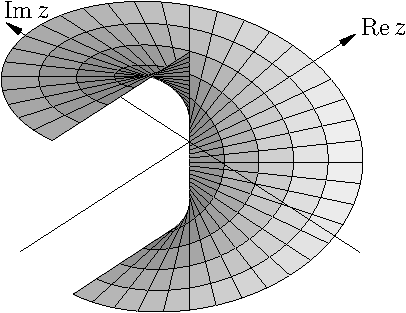
\includegraphics{figures/arggraph}
\caption{Grafik cabang utama argumen.\label{fig:arggraph}}
\end{myfig}
